%
% introduction.tex
%
% Copyright (C) 2021 by SpaceLab.
%
% Flatsat Platform Documentation
%
% This work is licensed under the Creative Commons Attribution-ShareAlike 4.0
% International License. To view a copy of this license,
% visit http://creativecommons.org/licenses/by-sa/4.0/.
%

%
% \brief Introduction chapter.
%
% \authors: Gabriel Mariano Marcelino <gabriel.marcelino@spacelab.ufsc.br> and Yan Castro de Azeredo <yan.azeredo@spacelab.ufsc.br>
%
% \institution Universidade Federal de Santa Catarina (UFSC)
%
% \version 0.2.0
%
% \date 2020/07/16
%

\chapter{Introduction} \label{ch:introduction}

The SpaceLab FlatSat Platform is a testbed for CubeSat PCB\nomenclature{\textbf{PCB}}{\textit{Printed Circuit Board.}} modules. FlatSats enable easier, faster and a secure method for testing subsystens independently while been integrated in a flat design before going to integration on a CubeSat form factor. The PCB can support up to 7 modules, all PC-104 pins are interligated to flexibilize its use, only the particularity connection between modules need to be be taken into account. One PC-104 has inverted pinout, the board also makes it possible to have two seperate power supplies, a UART\nomenclature{\textbf{UART}}{\textit{Universal Asynchronous Receiver/Transmitter.}} to USB\nomenclature{\textbf{USB}}{\textit{Universal Serial Bus.}} converter for 4 modules, kill-switches activation though SPDTs\nomenclature{\textbf{SPDT}}{\textit{Single Pole, Double Throw.}}, Remove Before Flight (RBF\nomenclature{\textbf{RBF}}{\textit{Remove Before Flight.}}) pin header, connector for charging batteries and SMA\nomenclature{\textbf{SMA}}{\textit{SubMiniature version A.}} connectors for antennas. This project is to be used on the GOLDS-UFSC mission \cite{golds-ufsc} during test phase.

\begin{figure}[!ht]
    \begin{center}
        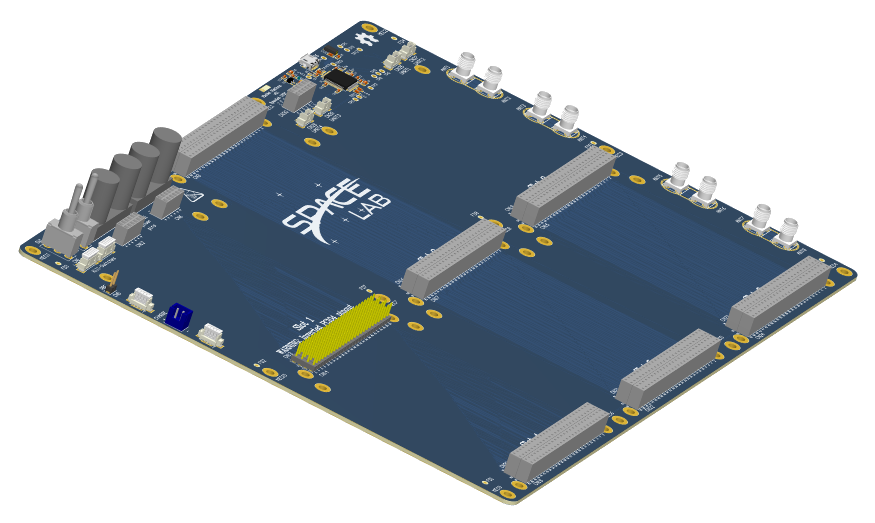
\includegraphics[width=0.75\textwidth]{figures/flatsat_perspective_image.png}
        \caption{3D view of the FlatSat PCB.}
        \label{fig:pcb-3d}
    \end{center}
\end{figure}

All the project, source and documentation files are available freely on a GitHub repository \cite{flatsat-platform-repo} under its respective licenses.
